\documentclass[preprint,12pt]{elsarticle}
% Target: Computer Networks (Elsevier). Every number in this file comes from paper/numbers.json or
% paper/tables/*.tex (generated by paper/analysis.py); every figure from paper/figures.py.
\usepackage[T1]{fontenc}
\usepackage[utf8]{inputenc}
\usepackage{amsmath,amssymb}
\usepackage{graphicx}
\usepackage{booktabs,multirow}
\usepackage{algorithm}
\usepackage{algpseudocode}
\usepackage[hidelinks]{hyperref}
\usepackage{xcolor}
\newcommand{\verify}[1]{\textcolor{black}{[VERIFY: #1]}}

\journal{Computer Networks}

\begin{document}
\begin{frontmatter}

\title{Choosing backup paths from hazard history: disaster-aware path selection for traffic-engineering recovery, tested on real cyclones and earthquakes}

\author[aids]{Uday Pratap Singh\corref{cor1}}
\ead{udaypratap@allduniv.ac.in}
\author[ce]{Bersha Kumari}
\author[ce]{Ebtasam Ahmad Siddiqui}
\cortext[cor1]{Corresponding author}
\affiliation[aids]{organization={Department of Artificial Intelligence and Data Science, Poornima Institute of Engineering and Technology},
            city={Jaipur}, postcode={302017}, state={Rajasthan}, country={India}}
\affiliation[ce]{organization={Department of Computer Engineering, Poornima Institute of Engineering and Technology},
            city={Jaipur}, postcode={302017}, state={Rajasthan}, country={India}}

\begin{abstract}
When a disaster cuts links in a backbone network, a traffic-engineering controller can only move traffic onto the backup paths it computed in advance. If a cyclone or earthquake destroys all of those paths together, the traffic is lost even though other routes still exist. We ask whether historical hazard records can tell an operator which backup paths to precompute. We present DART, a selection rule that keeps $k-1$ link-disjoint paths per demand pair and replaces the last one only when real past footprints show that the replacement would have survived more disasters. We built an evaluation framework that maps United States Geological Survey ShakeMap intensity grids, NOAA HURDAT2 tracks and IBTrACS typhoon wind radii onto seven real backbone topologies and measures recovery with a linear program. The method was developed on two networks, frozen, and then tested twice under criteria committed before each test. On 2{,}400 held-out geographic-disk failures in three unseen networks, DART lowered the mean routable traffic loss by 0.42 to 0.54 percentage points relative to edge-disjoint paths (Holm-corrected $p<10^{-42}$). On 211 real cyclone and earthquake footprints from 2018--2025 on seven networks, its mean loss was 0.16\% against 0.30\% for edge-disjoint paths; the rules tied in 162 events and DART lost less in 47 and more in 2 (Holm-corrected $p=8.6\times10^{-8}$). The gains are small in absolute terms: endpoints that a disaster isolates or destroys account for a mean loss of 12.4\% that no routing can recover, and earthquakes on national backbones broke too few links to separate any of the rules.
\end{abstract}

\begin{keyword}
traffic engineering \sep network reliability \sep geographically correlated failures \sep tropical cyclones \sep earthquakes \sep path selection
\end{keyword}

\end{frontmatter}

% =====================================================================================
\section{Introduction}
\label{sec:intro}

Backbone networks lose links to weather and ground motion every year. A tropical cyclone can cut power and fibre across several hundred kilometres, and an earthquake can sever ducts along a fault. Traffic engineering (TE) systems in wide-area networks usually split each demand pair's traffic over a small set of precomputed paths, or tunnels, and re-optimise that split when conditions change \cite{prete25,aegis26}. The re-optimisation is fast and, over the surviving tunnels, optimal. Its weak point is the tunnel set itself: when a disaster destroys every tunnel of a pair at once, the pair is cut off from the controller's point of view, even if the physical network still connects it.

Which tunnels fail together depends on geography. Two link-disjoint paths that run through the same coastal corridor are not independent when a hurricane makes landfall there. Geographically correlated failures have been studied for more than a decade, from vulnerability analysis of fibre and WDM networks \cite{neumayer11,agarwal13} to protection over shared-risk-link-group-disjoint geodiverse paths \cite{giraosilva20} and seismic reliability assessment \cite{jimenez23}. Learned TE has developed in parallel. Recent systems optimise TE directly from historical traffic demands \cite{dote23}, accelerate the TE optimisation with graph neural networks and reinforcement learning \cite{teal23}, transfer across changing topologies \cite{harp24,geminet26}, or reroute around multiple link failures with path-based graph neural networks \cite{pathgnn25}. These systems are usually evaluated with random or single-link failures and do not use the spatial record of real hazards.

This paper asks a narrow question: can the historical record of real cyclones and earthquakes improve the choice of TE backup paths, at a fixed tunnel budget, when the method is judged on disasters it has not seen? To answer it we combined three public archives of real hazard footprints with seven real backbone topologies, built a recovery evaluation that separates traffic no routing can save from traffic that a better tunnel set could have saved, and tested a simple selection rule under pre-registered criteria.

The contributions are as follows.
\begin{enumerate}
\item An evaluation framework that maps real hazard footprints onto real backbone topologies: USGS ShakeMap intensity grids \cite{trinet99}, NOAA HURDAT2 best tracks \cite{hurdat13} and IBTrACS typhoon wind radii \cite{ibtracs10}, selected by fixed rules rather than by hand. Real hurricanes have been used before to evaluate the resilience of real topologies \cite{alenazi23}; here three archives are used systematically, and lost traffic is split into an unservable part and a part that the choice of tunnels controls. Recovery is scored with an exact linear program, and lost traffic is split into an unservable part and a routable part (Section~\ref{sec:setup}).
\item DART (Disaster-Aware, Risk-learned Tunnel selection), a path-selection rule that keeps the classical link-disjoint backbone and changes the last tunnel only when real past footprints show a measurable benefit (Section~\ref{sec:method}). Geodiverse protection takes shared-risk groups as input \cite{giraosilva20}, and probabilistic TE models failure probabilities from failure data \cite{teavar19} or optical telemetry \cite{prete25}. DART instead estimates which links fail together from archived hazard footprints and uses that estimate to choose the tunnel set.
\item Two held-out tests whose criteria were committed to a public repository before they were run: synthetic geographic disks on three networks never used during development, and 211 real cyclone and earthquake footprints from 2018--2025 on seven networks (Section~\ref{sec:results}).
\item A report of what did not work and what the data cannot show: the first version of the method failed its pilot criterion, the absolute gains are small compared with the traffic that no routing can recover, and earthquakes did not discriminate between path rules on national backbones (Sections~\ref{sec:results} and \ref{sec:discussion}).
\end{enumerate}

We use the word ``learned'' in a narrow sense. DART estimates which tunnels fail together from data; it is not a neural network. We deliberately evaluated a transparent rule first, because a learned model is only worth building if the hazard record carries a signal that a simple rule can already exploit.

% =====================================================================================
\section{Related work}
\label{sec:related}

\paragraph{Traffic engineering under failures}
Forward fault correction (FFC) spreads traffic so that freedom from congestion is guaranteed under any combination of up to $k$ faults, such as link failures \cite{ffc14}. TeaVaR borrows from financial risk theory: it builds a probabilistic failure model from empirical data and maximises the bandwidth allocated to users subject to an operator-specified availability target \cite{teavar19}. PreTE predicts fibre cuts from optical-layer degradation, updates tunnels proactively and then reallocates traffic among them \cite{prete25}. AEGIS takes the opposite route to tunnel-based TE: it minimises the conditional value at risk of the total throughput loss over a set of failure situations with a linear program and avoids precomputed paths altogether, noting that tunnel-based TE is limited when only a few paths are precomputed and scales poorly when many are \cite{aegis26}. MetaOpt finds the performance gap between a heuristic, such as a production TE heuristic, and the optimum, together with the adversarial inputs that cause it \cite{metaopt24}. FFC and TeaVaR decide how much traffic to place on tunnels, PreTE also updates tunnels from predicted fibre cuts, and AEGIS avoids tunnels altogether. DART stays within tunnel-based TE and addresses the choice of which few tunnels exist, using hazard archives rather than per-element failure probabilities.

\paragraph{Learned traffic engineering}
DOTE learns TE configurations directly from historical demands \cite{dote23}. Teal combines a graph neural network with multi-agent reinforcement learning to accelerate TE optimisation in large wide-area networks \cite{teal23}. HARP \cite{harp24} and Geminet \cite{geminet26} target topologies that change, for example after link failures, and FIGRET makes TE robust to traffic bursts \cite{figret24}. PathGNN targets distributed TE, where each router chooses routes without a complete global view: it represents paths and the links they share as a bipartite graph, is trained by supervised learning on optimal routing strategies, and exchanges GNN messages among routers to make local routing decisions. On four real topologies its authors report at least 24.4\% better load balancing than distributed TE baselines, with lower end-to-end delay, under dynamic traffic and up to 35.3\% better performance under multiple link failures \cite{pathgnn25}. Other work applies multi-agent reinforcement learning with teacher--student distillation to QoS routing with link failures \cite{dts25}, or adversarial reinforcement learning to routing in space--air--ground networks \cite{rarl26}. Work on interpretability converts learned networking policies into decision trees \cite{metis20}, explains TE models with explainable-AI tools \cite{clearnet25}, or triages routing incidents from active measurements \cite{vasileva26}. To our knowledge, none of these evaluates path choice against real hazard footprints held out by time.

\paragraph{Disaster-resilient networks}
Geographically correlated failures were modelled as circles and line segments in early work on fibre vulnerability \cite{neumayer10,neumayer11} and as probabilistic regional failures in WDM networks \cite{agarwal13}. A special issue of \emph{Networks} collected optimisation problems on resilience to random failures and disaster-induced massive failures \cite{rak20}. Girão-Silva et al.\ quantify the extra path length and transponder cost of shared-risk-link-group-disjoint geodiverse protection relative to plain link-disjointness \cite{giraosilva20}. Andrés-Thió et al.\ augment networks in the plane with new links for resilience against disasters modelled as line segments \cite{andresthio22}, and Ferdousi et al.\ schedule progressive recovery of networks and data centres after large disasters \cite{ferdousi20}. In wireless and emergency settings, routing has been adapted to infrastructure failures with federated reinforcement distillation \cite{fedrdr24}, and game-theoretic SDN routing has been compared with static routing on Abilene under single-link and correlated failures \cite{sreeveda26}. Du studied the implications of 5G roll-out for the post-earthquake functionality of regional telecommunication infrastructure \cite{du24}. Two recent studies use real hazards. Alenazi evaluates the physical topologies of four large United States providers against Hurricanes Ivan and Katrina with topological robustness metrics and weather data \cite{alenazi23}, and Jiménez et al.\ estimate post-earthquake element states with probabilistic seismic hazard analysis and fragility curves to compute network reliability \cite{jimenez23}. Both assess resilience; we use archived footprints of many events to choose TE tunnels and test that choice on later events.

\paragraph{Quantum optimisation for routing}
Near-term quantum algorithms have been applied to multi-objective routing \cite{chiew24,bouchmal25}, to routing and wavelength assignment with shared-risk avoidance \cite{davies25}, and to latency-resilient routing under dual-link failures on a five-node example \cite{harb26}. These studies demonstrate formulations at small scale. We did not use quantum hardware, because the tunnel-selection and recovery problems at our scale are solved exactly by classical linear programming.

Table~\ref{tab:related} summarises how the closest lines of work differ from this study. The distinguishing combination is the use of real hazard footprints both for choosing tunnels and for a time-separated test.

\begin{table}[t]
\centering
\caption{Positioning against the closest published work. ``Real footprints'' means archived spatial records of actual hazards; ``held out by time'' means the method is evaluated on events later than those it used.}
\label{tab:related}
\small
\resizebox{\linewidth}{!}{\begin{tabular}{p{4.6cm}p{2.2cm}p{2.4cm}p{2.2cm}p{2.0cm}}
\toprule
Work & Decides tunnel set & Correlated failures & Real hazard footprints & Held out by time \\
\midrule
FFC \cite{ffc14} & no & $k$ arbitrary & no & -- \\
TeaVaR \cite{teavar19} & no & empirical failure model & no & -- \\
PreTE \cite{prete25} & tunnels updated & fibre degradation & optical telemetry & -- \\
AEGIS \cite{aegis26} & no tunnels & failure situations & no & -- \\
Learned TE \cite{dote23,teal23,harp24,geminet26,pathgnn25} & no & random single or multiple & no & -- \\
Geodiverse protection \cite{giraosilva20} & yes & shared-risk groups & no & -- \\
Geographic failure models \cite{neumayer11,agarwal13} & analysis & geometric & no & -- \\
Hurricane evaluation \cite{alenazi23} & no (assessment) & hurricanes & yes (2 events) & -- \\
Seismic reliability \cite{jimenez23} & no (assessment) & seismic hazard model & no & -- \\
This work (DART) & yes & from archives & yes & yes \\
\bottomrule
\end{tabular}}
\end{table}

% =====================================================================================
\section{Problem formulation}
\label{sec:problem}

A backbone is a graph $G=(V,E)$ in which every undirected link $e\in E$ provides two directed arcs with the same capacity $c_e$ (Mbit/s). The demand from $s$ to $t$ is $D_{st}\ge 0$. A TE controller precomputes, for each pair $(s,t)$ with $D_{st}>0$, a set $\mathcal{P}_{st}$ of at most $k$ loop-free paths and splits $D_{st}$ over them with ratios $x_{st,p}$.

A failure scenario $\omega$ removes a set of nodes $V_\omega$ and links $E_\omega$; a link also fails when one of its endpoints fails. A pair is \emph{servable} under $\omega$ if neither endpoint failed and the endpoints remain connected in $G-V_\omega-E_\omega$. Traffic of unservable pairs is lost under any routing:
\begin{equation}
U_\omega=\sum_{(s,t)\ \text{not servable}} D_{st}.
\label{eq:unservable}
\end{equation}
For a servable pair, let $\mathcal{P}^{\omega}_{st}\subseteq\mathcal{P}_{st}$ be the precomputed paths that survive. After a failure the controller re-solves the split ratios over the surviving paths to minimise the maximum link utilisation (MLU):
\begin{align}
\min_{x,\,u}\ & u \label{eq:lp}\\
\text{s.t.}\ & \sum_{p\in\mathcal{P}^{\omega}_{st}} x_{st,p}=1 && \forall (s,t)\in S^\omega_{+}, \label{eq:lp-demand}\\
& \sum_{(s,t)}\ \sum_{p\in\mathcal{P}^{\omega}_{st}:\,a\in p} D_{st}\,x_{st,p}\le u\,c_a && \forall a\in A\setminus A_\omega, \label{eq:lp-cap}\\
& x_{st,p}\ge 0, \nonumber
\end{align}
where $S^\omega_{+}$ is the set of servable pairs with at least one surviving path and $A_\omega$ the failed arcs. Constraint~\eqref{eq:lp-demand} routes all demand of these pairs and constraint~\eqref{eq:lp-cap} bounds every surviving arc's utilisation by $u$. Servable pairs whose paths have all failed cannot be served by the controller even though the physical network still connects them. Their demand is the \emph{routable loss}, the quantity that the choice of $\mathcal{P}$ controls:
\begin{equation}
R_\omega(\mathcal{P})=\sum_{(s,t)\ \text{servable}:\ \mathcal{P}^{\omega}_{st}=\emptyset} D_{st}.
\label{eq:routable}
\end{equation}
We report $U_\omega$ and $R_\omega$ as fractions of total demand. To describe the tail of $R_\omega$ over a set of $n$ scenarios we use the conditional value at risk at level $\alpha=0.95$ \cite{cvar00}, computed empirically as the mean of the $\lceil(1-\alpha)n\rceil$ largest values:
\begin{equation}
\mathrm{CVaR}_{0.95}(R)=\frac{1}{\lceil 0.05\,n\rceil}\sum_{i=1}^{\lceil 0.05\,n\rceil} R_{(i)},
\label{eq:cvar}
\end{equation}
where $R_{(1)}\ge R_{(2)}\ge\dots$ are the sorted losses. The tunnel-selection problem is to choose $\mathcal{P}$, with $|\mathcal{P}_{st}|\le k$, so that future disasters produce small routable loss without raising the MLU in normal operation.

% =====================================================================================
\section{DART: tunnel selection from hazard history}
\label{sec:method}

\subsection{Failure footprints}
\label{sec:footprints}

Each link is modelled as the great-circle arc between its endpoints, sampled every $\delta=10$~km. A node fails if its location lies inside a footprint $\Phi$; a link fails if any of its sample points does. Three footprint types are used.

\emph{Earthquakes.} ShakeMap estimates shaking over a whole region by spatially interpolating recorded ground motions and converting them to intensity \cite{trinet99}; the USGS distributes the result as a grid of modified Mercalli intensity $I(\mathbf{z})$ at points $\mathbf{z}$ of a regular latitude--longitude grid. The footprint at threshold $\theta$ is
\begin{equation}
\Phi^{\mathrm{eq}}_{\theta}=\{\mathbf{z}: I(\mathbf{z})\ge\theta\},
\label{eq:eq}
\end{equation}
with $\theta=\mathrm{VII}$ (primary) and $\theta=\mathrm{VIII}$ (secondary). Points outside the grid extent are treated as undamaged.

\emph{Tropical cyclones.} HURDAT2 \cite{hurdat13} and IBTrACS \cite{ibtracs10} give, every six hours, the storm centre $\mathbf{c}_\tau$ and the radius $r^{q}_{\tau,v}$ (nautical miles, converted to km) to which winds of at least $v$ knots extend in each compass quadrant $q\in\{\mathrm{NE},\mathrm{SE},\mathrm{SW},\mathrm{NW}\}$. We interpolate centres and radii to one-hour steps and define
\begin{equation}
\Phi^{\mathrm{tc}}_{v}=\bigcup_{\tau}\ \{\mathbf{z}: d(\mathbf{c}_\tau,\mathbf{z})\le r^{q(\mathbf{c}_\tau,\mathbf{z})}_{\tau,v}\},
\label{eq:tc}
\end{equation}
where $d$ is the great-circle distance and $q(\cdot)$ the quadrant of the bearing from the centre to $\mathbf{z}$. We use $v=34$~kt (primary) and $v=64$~kt (secondary). Track rows without radii are dropped, and gaps longer than 12~h are not bridged, so no footprint is invented between distant observations.

\emph{Geographic disks.} For training and for the synthetic test we draw disks of radius $\rho\in\{50,100,200,400\}$~km with centres uniform in the bounding box of the network expanded by one degree, keeping only disks that fail at least one element \cite{neumayer11}.

Whether an element inside a footprint really fails depends on construction, power backup and other factors that public data do not record. The rule above is therefore an assumption, and we test two thresholds for each hazard to see whether the conclusions depend on it.

\subsection{Selection rule}
\label{sec:rule}

Let $\Omega$ be a set of training scenarios with weights $w_\omega\ge 0$. In Test~2 (Section~\ref{sec:protocol}) $\Omega$ contains every real event before 2018 that fails at least one element of the network plus 800 random disks, and each of the three families (cyclones, earthquakes, disks) receives a total weight of one, shared equally among its scenarios. For a pair $(s,t)$, a set of paths $Q$ and a candidate path $p$, the \emph{coverage gain} of $p$ is the weight of training scenarios in which the pair is not destroyed at an endpoint, no path in $Q$ survives, and $p$ survives:
\begin{equation}
g_{st}(p\mid Q)=\sum_{\omega\in\Omega} w_\omega\,\mathbb{1}[s,t\notin V_\omega]\ \mathbb{1}[Q\cap\mathcal{S}_\omega=\emptyset]\ \mathbb{1}[p\in\mathcal{S}_\omega],
\label{eq:gain}
\end{equation}
where $\mathcal{S}_\omega$ is the set of paths with no failed arc in $\omega$. DART builds $\mathcal{P}_{st}$ in two steps (Algorithm~\ref{alg:dart}).
\begin{enumerate}
\item \emph{Backbone.} Take the shortest path by hop count, remove its links, and repeat until $k-1$ mutually link-disjoint paths are found or the pair is disconnected. This is a greedy form of the classical disjoint-path construction \cite{suurballe74}; it protects every pair against any single link failure on its backbone paths.
\item \emph{Last tunnel.} Let $Q$ be the backbone and $p^{\mathrm{ed}}$ the path that the edge-disjoint rule would add next (another disjoint path or, if none exists, the next-shortest path \cite{yen71}). Among candidate paths $C_{st}$ (up to 32 loop-free paths no longer than three times the shortest in kilometres), DART chooses
\begin{equation}
p^{\star}=\begin{cases}\arg\max_{p\in C_{st}} g_{st}(p\mid Q) & \text{if } \max_{p\in C_{st}} g_{st}(p\mid Q)>g_{st}(p^{\mathrm{ed}}\mid Q),\\ p^{\mathrm{ed}} & \text{otherwise,}\end{cases}
\label{eq:replace}
\end{equation}
breaking ties by fewest links shared with $Q$ and then by hop count.
\end{enumerate}
The rule changes the classical choice only where the hazard record supports a change. Where the record is silent, DART reduces to edge-disjoint selection. Equation~\eqref{eq:gain} is a weighted coverage function, which is monotone and submodular \cite{nemhauser78}. With a single free tunnel, Eq.~\eqref{eq:replace} maximises it exactly over the candidate set.

\begin{algorithm}[t]
\caption{DART tunnel selection for one demand pair $(s,t)$}
\label{alg:dart}
\begin{algorithmic}[1]
\Require graph $G$, budget $k$, candidates $C_{st}$, training scenarios $\Omega$ with weights $w$
\State $Q\gets\emptyset$; $H\gets G$
\While{$|Q|<k-1$ \textbf{and} $s,t$ connected in $H$}
  \State $p\gets$ shortest $s$--$t$ path in $H$ by hops; $Q\gets Q\cup\{p\}$; remove links of $p$ from $H$
\EndWhile
\State $p^{\mathrm{ed}}\gets$ next path chosen by the edge-disjoint rule
\State $p^{+}\gets\arg\max_{p\in C_{st}} g_{st}(p\mid Q)$ \Comment{Eq.~\eqref{eq:gain}}
\If{$g_{st}(p^{+}\mid Q)>g_{st}(p^{\mathrm{ed}}\mid Q)$} \Return $Q\cup\{p^{+}\}$ \Else\ \Return $Q\cup\{p^{\mathrm{ed}}\}$ \EndIf
\end{algorithmic}
\end{algorithm}

The cost of the rule is dominated by evaluating survival of $|C_{st}|$ candidates in $|\Omega|$ scenarios for every pair, $O(|V|^2\,|C|\,|\Omega|\,\ell)$ with $\ell$ the path length. Selection is computed once, offline. The online step after a disaster is the linear program of Eqs.~\eqref{eq:lp}--\eqref{eq:lp-cap}, which is identical for every selection rule, so DART adds no online cost. Figure~\ref{fig:pipeline} shows the offline and online stages.

\begin{figure}[t]
\centering
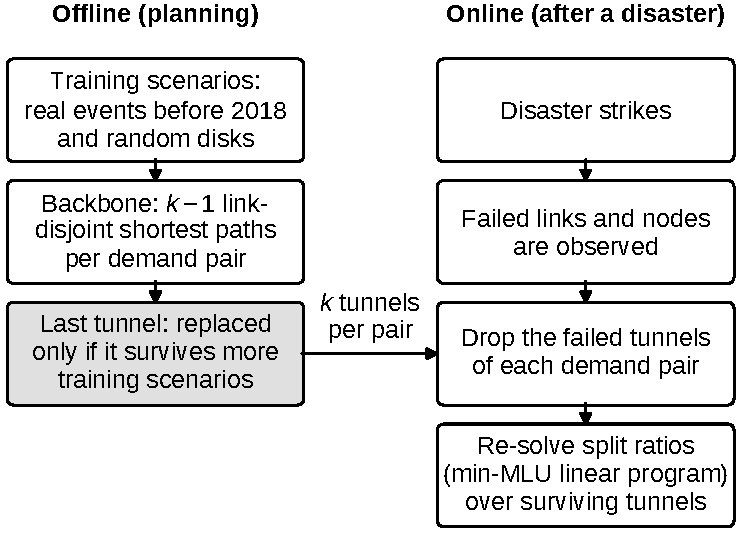
\includegraphics[width=\linewidth]{figs/fig1_pipeline.pdf}
\caption{DART. Offline, training failure scenarios from real events before 2018 and random disks decide whether the last of the $k$ tunnels of each pair should differ from the classical edge-disjoint choice. Online, the controller drops failed tunnels and re-solves split ratios with the linear program of Eqs.~(\ref{eq:lp})--(\ref{eq:lp-cap}).}
\label{fig:pipeline}
\end{figure}

The upper row of Fig.~\ref{fig:pipeline} is the only place where hazard data enter. Training failure scenarios are reduced to sets of failed links, and DART uses them only to decide the last tunnel. The lower row is the standard re-optimisation that every compared rule uses. This separation is deliberate: any difference in the results comes from which tunnels exist, not from how traffic is split over them.

% =====================================================================================
\section{Experimental setup}
\label{sec:setup}

\subsection{Networks and demand}
We used seven real topologies with geographic coordinates from the Internet Topology Zoo \cite{topozoo11}, as distributed by TopoHub \cite{topohub23}: AttMpls and BtNorthAmerica (United States), G\'EANT (Europe), IIJ (Japan), CERNET (China), GARR (Italy) and GRNET (Greece). Two further networks, Abilene (with capacities and the demand matrix of SNDlib \cite{sndlib10}) and BellSouth, were used only for development (Section~\ref{sec:protocol}). Topology Zoo records neither capacities nor traffic, so we assumed a uniform capacity of 10~Gbit/s per link and a gravity demand model in which node mass equals node degree. Demand was scaled so that the optimal MLU without failures equals 0.6. Under this scaling the MLU values are relative; the routable-loss fractions we report do not depend on the scale. Table~\ref{tab:data} lists the networks and the number of real events that fail at least one of their elements.

\begin{table}[t]
\centering
\caption{Test networks and real-event scenarios at the primary thresholds (34-kt winds, MMI VII). Each entry counts events that fail at least one node or link of that network. Training events (before 2018) were used only to select tunnels; test events (2018--2025) only to evaluate them.}
\label{tab:data}
\small
\resizebox{\linewidth}{!}{\begin{tabular}{lrrrrrr}
\toprule
 & & & \multicolumn{2}{c}{Training (before 2018)} & \multicolumn{2}{c}{Test (2018--2025)} \\
\cmidrule(lr){4-5}\cmidrule(lr){6-7}
Network & Nodes & Links & Cyclones & Earthquakes & Cyclones & Earthquakes \\
\midrule
AttMpls & 25 & 56 & 44 & 4 & 37 & 0 \\
BtNorthAmerica & 33 & 70 & 46 & 1 & 41 & 1 \\
G\'EANT & 37 & 58 & 11 & 6 & 12 & 2 \\
IIJ & 28 & 54 & 133 & 7 & 71 & 2 \\
CERNET & 37 & 54 & 101 & 0 & 42 & 0 \\
GARR & 48 & 62 & 0 & 1 & 1 & 0 \\
GRNET & 34 & 39 & 0 & 3 & 0 & 2 \\
\midrule
Total & & & 335 & 22 & 204 & 7 \\
\bottomrule
\end{tabular}
}
\end{table}

Table~\ref{tab:data} shows that the real-event evidence is uneven. IIJ and CERNET carry most of the typhoon scenarios, the two United States networks most of the Atlantic hurricanes, and the Mediterranean networks only a handful of events. Earthquakes are rare in both periods: seven test scenarios over all networks. The pooled analysis below therefore speaks mainly about tropical cyclones.

\subsection{Hazard data and event selection}
Cyclone tracks came from HURDAT2 for the Atlantic (seasons 2004 onward, when wind radii are available) \cite{hurdat13} and from IBTrACS v04r01 for the western Pacific (2001 onward, United States agency radii) \cite{ibtracs10}. Earthquakes were every USGS ComCat event of magnitude 6.0 or more between 1990 and 2025 with a ShakeMap, whose epicentre lay within the network's bounding box expanded by two degrees and within 300~km of a link. The 300~km filter only limited downloads: at these magnitudes intensity VII rarely extends farther. Footprints follow Eq.~\eqref{eq:eq} for earthquakes and Eq.~\eqref{eq:tc} for cyclones. Events were split by year: before 2018 for training, 2018--2025 for testing. No event was chosen by hand, and every downloaded file is recorded with its SHA-256 checksum.

\subsection{Compared rules and metrics}
All rules choose $k=4$ tunnels per pair and share the first path (shortest by hops). \emph{Shortest paths} takes the four shortest simple paths by hop count \cite{yen71}. \emph{Edge-disjoint} repeats shortest-path search after removing used links and fills with shortest paths when no disjoint path remains (greedy disjoint construction, cf.\ \cite{suurballe74}). \emph{Geo-diverse} adds, at each step, the candidate with the fewest link points within 50~km of already chosen paths, a data-free form of geographic diversity in the spirit of \cite{giraosilva20}. We also report shortest paths with $k=8$ as a reference with twice the tunnel budget. The primary metric is the routable loss $R_\omega$ of Eq.~\eqref{eq:routable}; we also report its 95th percentile, $\mathrm{CVaR}_{0.95}$ (Eq.~\eqref{eq:cvar}), its maximum, the unservable loss $U_\omega$ (Eq.~\eqref{eq:unservable}) and the MLU without failures. Linear programs were solved with HiGHS \cite{highs18} through SciPy \cite{scipy20}; paths were computed with NetworkX \cite{networkx08}.

\subsection{Development and testing protocol}
\label{sec:protocol}
The method was developed on Abilene and BellSouth only. A first version that chose all backup tunnels by coverage failed its pre-registered pilot criterion on both networks: on held-out natural scenarios (2018--2024 storms and random disks) it lost more traffic than edge-disjoint paths in more scenarios than it saved, and it raised the no-failure MLU on BellSouth by 26\%. Three revisions followed, each motivated by a diagnosed failure case; the full history is in Supplementary Section~S1. The fourth version (Section~\ref{sec:rule}) was then frozen and tested twice, each time under a criterion committed to the public repository before the test was run (Supplementary Section~S2).

\emph{Test 1 (unseen networks):} AttMpls, BtNorthAmerica and G\'EANT, none of which was used during development. Training scenarios were the pre-2018 events of a fixed list of 12 Atlantic hurricanes and 10 earthquakes plus 800 random disks; the test set was 800 fresh random disks per network plus the post-2018 events of the same list (15, 17 and 3 real scenarios). The criterion was evaluated on this combined natural test set, of which 98\% were disks; below we report the disks, and the real events are analysed with systematic selection in Test~2. \emph{Test 2 (real events):} all 211 primary-threshold test scenarios of Table~\ref{tab:data}. In both tests the confirmatory statistic was the paired two-sided Wilcoxon signed-rank test \cite{wilcoxon45} of DART against each classical rule on per-scenario routable loss, with Holm correction across the three comparisons \cite{holm79}. We report mean paired differences with 10{,}000-resample bootstrap 95\% confidence intervals and the matched-pairs rank-biserial correlation $r_{\mathrm{rb}}$ (positive values favour DART).

While preparing this manuscript we found that the linear-programming solver leaves split ratios that sum to one only up to about $10^{-16}$, which produced spurious ``losses'' of that size in 410 of 1{,}335 real-event results. The smallest genuine loss was $3.1\times10^{-4}$ of demand. We therefore set values below $10^{-9}$ to zero. The pre-registered tests compared raw values; their conclusions are unchanged under either treatment, and both versions are reported in Supplementary Section~S3.

% =====================================================================================
\section{Results}
\label{sec:results}

\subsection{Held-out geographic disks}

Table~\ref{tab:disk} reports the disk scenarios of Test~1; the pre-registered criterion, evaluated on all natural test scenarios, was met on all three networks (Supplementary Section~S2). On each of the three networks DART had the lowest mean, 95th-percentile and $\mathrm{CVaR}_{0.95}$ routable loss of the four $k=4$ rules, and all nine paired comparisons were significant after Holm correction (largest $p_{\mathrm{Holm}}=1.1\times10^{-11}$). Against edge-disjoint paths, the mean loss fell from 0.94\% to 0.48\% on AttMpls, from 1.02\% to 0.48\% on BtNorthAmerica and from 0.74\% to 0.32\% on G\'EANT. The rank-biserial correlations against edge-disjoint paths were between 0.95 and 0.97: when the two rules differed, DART almost always lost less. The worst single disk is a different matter. On AttMpls the geo-diverse rule had the smallest worst-case loss (19.7\% against 23.2\% for DART), so the improvement concerns the bulk and the upper tail of the distribution rather than the single most damaging disk.

\begin{table}[t]
\centering
\caption{Test 1: routable loss on 800 held-out random disks per network (three networks not used during development). Mean difference is DART minus the rule in percentage points; $p_{\mathrm{Holm}}$ from paired two-sided Wilcoxon tests with Holm correction over the three comparisons per network; $r_{\mathrm{rb}}$ is the rank-biserial correlation (positive favours DART).}
\label{tab:disk}
\small
\resizebox{\linewidth}{!}{\begin{tabular}{llrrrrrr}
\toprule
Network & Rule & Mean (\%) & CVaR$_{0.95}$ (\%) & Worst (\%) & Mean diff. (pp) & $p_{\mathrm{Holm}}$ & $r_{\mathrm{rb}}$ \\
\midrule
\multirow{4}{*}{AttMpls ($n=800$)} & Shortest paths & 2.08 & 14.05 & 29.34 & -1.60 & $<10^{-15}$ & 0.99 \\
 & Geo-diverse & 0.85 & 7.38 & 19.72 & -0.37 & $<10^{-15}$ & 0.75 \\
 & Edge-disjoint & 0.94 & 9.74 & 26.85 & -0.46 & $<10^{-15}$ & 0.95 \\
 & DART & 0.48 & 5.89 & 23.21 & -- & -- & -- \\
\midrule
\multirow{4}{*}{BtNorthAmerica ($n=800$)} & Shortest paths & 2.14 & 15.16 & 30.64 & -1.66 & $<10^{-15}$ & 1.00 \\
 & Geo-diverse & 0.92 & 11.02 & 26.30 & -0.44 & $<10^{-15}$ & 0.71 \\
 & Edge-disjoint & 1.02 & 11.05 & 28.32 & -0.54 & $<10^{-15}$ & 0.97 \\
 & DART & 0.48 & 7.61 & 25.25 & -- & -- & -- \\
\midrule
\multirow{4}{*}{G\'EANT ($n=800$)} & Shortest paths & 1.32 & 15.57 & 34.98 & -0.99 & $<10^{-15}$ & 1.00 \\
 & Geo-diverse & 0.43 & 7.75 & 30.67 & -0.11 & $1.1\times10^{-11}$ & 0.62 \\
 & Edge-disjoint & 0.74 & 12.07 & 29.55 & -0.42 & $<10^{-15}$ & 0.97 \\
 & DART & 0.32 & 6.00 & 25.52 & -- & -- & -- \\
\bottomrule
\end{tabular}
}
\end{table}

Figure~\ref{fig:disk} shows the same tail measure across networks. The ordering of the classical rules is not stable: geo-diverse paths beat edge-disjoint paths in the tail on AttMpls and G\'EANT and are level with them on BtNorthAmerica (11.0\% against 11.1\%). DART is lowest on all three, at 5.9\%, 7.6\% and 6.0\%. Doubling the tunnel budget to eight shortest paths gave a $\mathrm{CVaR}_{0.95}$ of 9.9\%, 9.5\% and 9.7\%, all higher than DART with four tunnels.

\begin{figure}[t]
\centering
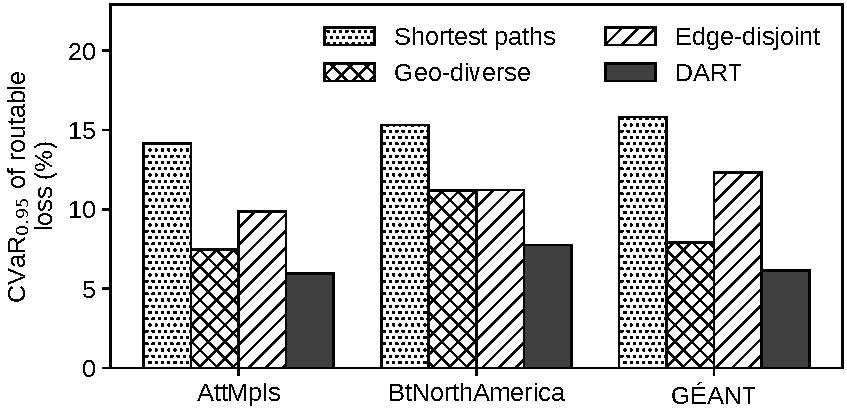
\includegraphics[width=\linewidth]{figs/fig5_disk_cvar.pdf}
\caption{Test 1: conditional value at risk ($\mathrm{CVaR}_{0.95}$, mean of the worst 5\% of scenarios) of routable loss on 800 held-out random disks per network, for four tunnel-selection rules with $k=4$.}
\label{fig:disk}
\end{figure}

These disks come from the same random model as the training disks, so Test~1 shows that DART generalises to new draws of a known failure distribution on unseen networks. It does not show that the hazard archives help. That question is answered by Test~2.

\subsection{Real cyclones and earthquakes, 2018--2025}

Table~\ref{tab:real} reports Test~2. Pooled over the seven networks, DART's mean routable loss was 0.16\% of demand, against 0.30\% for edge-disjoint paths, 0.53\% for geo-diverse paths and 0.64\% for shortest paths. The pre-registered criterion was met: the mean paired difference was negative and significant after Holm correction against each classical rule ($p_{\mathrm{Holm}}\le1.7\times10^{-6}$). The confidence intervals exclude zero. Against edge-disjoint paths the difference was $-0.13$ percentage points (95\% CI $-0.20$ to $-0.08$).

\begin{table}[t]
\centering
\caption{Test 2: routable loss on 211 real test scenarios (2018--2025, 34-kt winds or MMI VII) pooled over seven networks. B/W/T counts scenarios in which DART lost less, lost more, or tied. Other notation as in Table~\ref{tab:disk}.}
\label{tab:real}
\scriptsize
\resizebox{\linewidth}{!}{\begin{tabular}{lrrrrlrrr}
\toprule
 & \multicolumn{4}{c}{Routable loss (\% of demand)} & \multicolumn{4}{c}{DART minus rule (paired)} \\
\cmidrule(lr){2-5}\cmidrule(lr){6-9}
Rule ($k=4$ unless stated) & Mean & P95 & CVaR$_{0.95}$ & Worst & Mean diff. [95\% CI] & B/W/T & $p_{\mathrm{Holm}}$ & $r_{\mathrm{rb}}$ \\
\midrule
Shortest paths & 0.63 & 4.17 & 6.07 & 15.78 & -0.47 [-0.63, -0.32] & 67/1/143 & $1.0\times10^{-11}$ & 0.97 \\
Geo-diverse & 0.53 & 4.11 & 6.74 & 13.26 & -0.37 [-0.57, -0.20] & 41/6/164 & $1.7\times10^{-6}$ & 0.80 \\
Edge-disjoint & 0.30 & 1.98 & 3.61 & 8.32 & -0.13 [-0.20, -0.08] & 47/2/162 & $8.6\times10^{-8}$ & 0.90 \\
Shortest paths, $k=8$ & 0.21 & 1.14 & 3.24 & 12.56 & -- & -- & -- & -- \\
DART & 0.16 & 1.05 & 2.86 & 8.16 & -- & -- & -- & -- \\
\bottomrule
\end{tabular}
}
\end{table}

The counts in Table~\ref{tab:real} show the shape of the effect. In 162 of 211 scenarios DART and the edge-disjoint rule lost exactly the same traffic, usually none. In the remaining 49, DART lost less in 47 and more in 2. Most real events are survivable by any reasonable tunnel set; the hazard record helps in a minority of events, and in those it helps consistently. Figure~\ref{fig:exceed} gives the full distribution. DART lost no routable traffic in 90\% of events, against 76\% for edge-disjoint paths and 68\% for shortest paths, and its curve lies below the others at most loss levels. The curves meet near the largest losses, around 8\%, where the worst single events affect all rules similarly.

\begin{figure}[t]
\centering
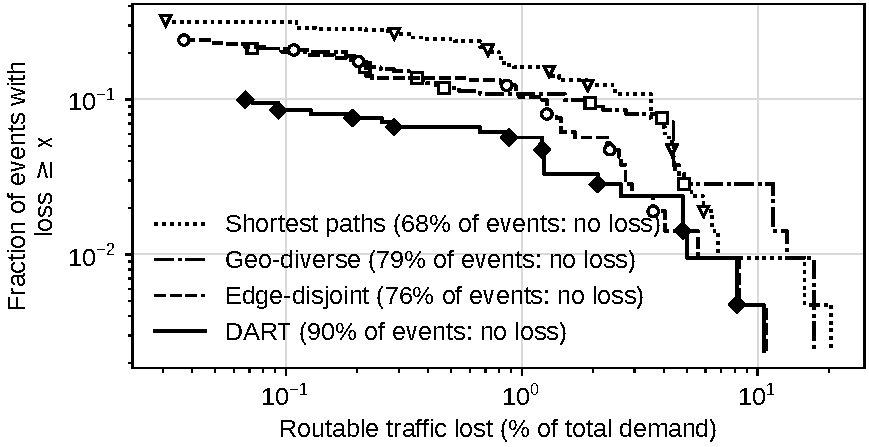
\includegraphics[width=\linewidth]{figs/fig3_real_exceedance.pdf}
\caption{Test 2: fraction of the 211 real test scenarios in which the routable loss reached at least the value on the horizontal axis (both axes logarithmic). Scenarios with no loss are not shown on the logarithmic axis; their share is given in the legend.}
\label{fig:exceed}
\end{figure}

Two robustness checks fixed in advance gave the same conclusion. A single storm can hit several networks, so the 211 scenarios are not independent. Averaging each event over the networks it hit left 141 events; DART was never worse than edge-disjoint paths and better in 36 of them ($p_{\mathrm{Holm}}=3.3\times10^{-7}$). At the stricter thresholds (64-kt winds, MMI VIII; 56 scenarios) DART was better than edge-disjoint paths in 10 scenarios, worse in none and tied in 46 ($p_{\mathrm{Holm}}=0.005$). With fewer and smaller footprints, the effect is smaller there: a mean of 0.23\% against 0.28\%.

Figure~\ref{fig:topo} breaks the result down by network. Among the $k=4$ rules, DART had the lowest mean loss on AttMpls, CERNET and IIJ. On BtNorthAmerica and G\'EANT the geo-diverse rule was slightly lower (0.06\% against 0.07\%, and 0.36\% against 0.37\%). The geo-diverse rule is unstable in the other direction: on IIJ it had by far the highest loss (1.14\%), because typhoons pass along the main Japanese corridor, which geographically separated detours in that topology do not avoid. Neither GRNET (two events) nor GARR (one event) lost routable traffic under any rule.

\begin{figure}[t]
\centering
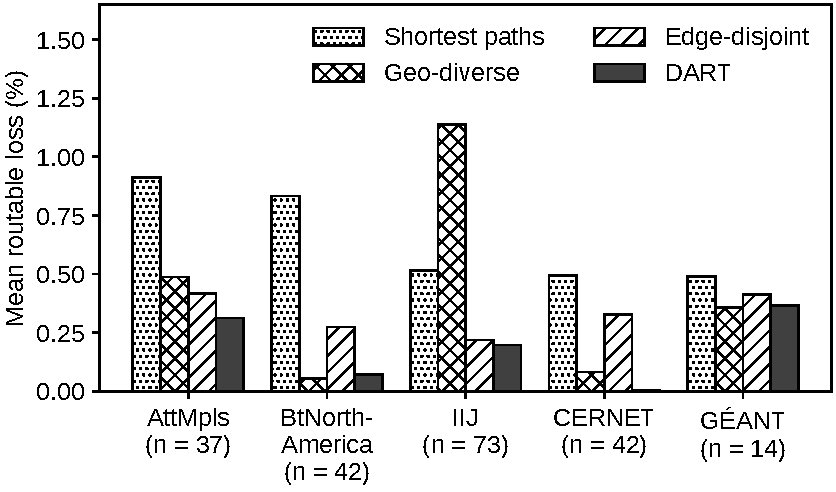
\includegraphics[width=\linewidth]{figs/fig4_real_by_topology.pdf}
\caption{Test 2 by network: mean routable loss over the real test scenarios of each network ($n$ below each name). GRNET ($n=2$) and GARR ($n=1$) had no routable loss under any rule and are omitted.}
\label{fig:topo}
\end{figure}

Figure~\ref{fig:footprints} shows the event with the most failed links in the test period on two networks. Hurricane Zeta (2020) failed 19 links and six nodes of AttMpls as it crossed the south-eastern United States, and Typhoon Jongdari (2018) failed 46 of the 54 links of IIJ. The second case explains why IIJ dominates the cyclone evidence: its nodes cluster around Tokyo and Osaka, so a single storm on an unusual westward track can take out most of the network. In such events much of the lost traffic is unservable, and tunnel selection can only change what happens to pairs whose endpoints survive.

\begin{figure}[t]
\centering
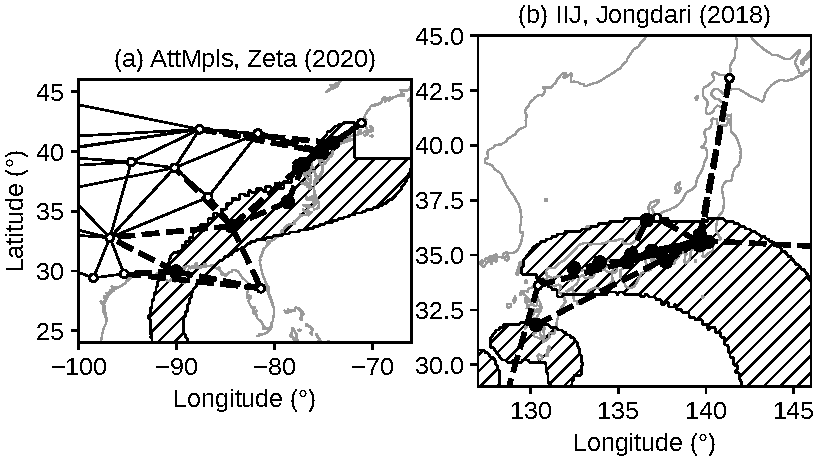
\includegraphics[width=\linewidth]{figs/fig2_footprints.pdf}
\caption{Real test events with the most failed links. Hatched: 34-kt wind footprint from the best track. Thick dashed lines: failed links; filled circles: failed nodes; grey: coastline. (a) AttMpls, Hurricane Zeta (2020). (b) IIJ, Typhoon Jongdari (2018); the trans-Pacific links of IIJ leave the map to the east.}
\label{fig:footprints}
\end{figure}

\subsection{Earthquakes and worst-case link cuts}

No real test earthquake produced routable loss under any rule. The seven test scenarios failed one or two links each (and one node, on the Greek island of Samos in GRNET), and every rule kept a surviving tunnel for every servable pair. Earthquakes therefore neither support nor contradict DART in this study.

As a secondary check we enumerated all cuts of one and two links on the Test~1 networks. DART had the lowest 95th-percentile routable loss on all three networks and the lowest worst case on AttMpls (1.8\%) and G\'EANT (9.8\% against 12.3\% for edge-disjoint paths). On BtNorthAmerica edge-disjoint paths had a lower worst case (3.9\% against 4.4\%). Supplementary Table~S4 gives the full numbers.

% =====================================================================================
\section{Discussion}
\label{sec:discussion}

\paragraph{What the hazard record adds}
Edge-disjointness already protects against any single link failure, which is why the classical rule and DART tie in most real events. The record of past cyclones adds information about which links tend to fail \emph{together}, for example two disjoint paths that both run along a hurricane-prone coast. DART only acts on that information when it is present, and it did not make a pair worse than the edge-disjoint choice in any event-level comparison of Test~2. This conservatism is the main lesson of the development history: the first version, which chose all backup tunnels from the hazard record, overfitted the training footprints and failed its pilot.

\paragraph{Size of the effect}
The improvements are statistically clear and practically small. A mean routable loss of 0.16\% instead of 0.30\% means that, for a backbone carrying 1~Tbit/s, about 1.3~Gbit/s more traffic stays reachable after an average test event. The mean unservable loss in the same scenarios was 12.4\%, roughly 77 times DART's routable loss. For operators, the larger lever against cyclones is therefore the topology itself (redundant links at stub nodes and away from shared corridors \cite{andresthio22}) and power backup at sites, not tunnel choice. Tunnel choice is cheap, though: DART adds no online computation, and on the three networks of Test~1 its no-failure MLU equalled the optimum of 0.6.

\paragraph{Earthquakes}
Intensity VII or more from magnitude 6--7 events covers a few tens of kilometres. National backbone links are hundreds of kilometres long and nodes are far apart, so the test earthquakes failed one or two links and no rule lost routable traffic. Where losses occurred they were unservable, at nodes attached by a single link. Testing tunnel selection against earthquakes would need regional or metropolitan networks, where one event can affect many elements; a seismic risk study of a regional 5G infrastructure, for example, projected significant performance degradation after major earthquakes \cite{du24}.

\paragraph{Limitations}
Several assumptions limit what these results show. (i) Links are drawn as great-circle arcs, while real fibre follows roads, railways and coasts. (ii) An element fails if it is inside a footprint, which ignores hardening and backup power; two thresholds per hazard only partly address this, and fragility curves, as used for earthquakes by Jiménez et al.\ \cite{jimenez23}, would be a more realistic damage model. (iii) Topology Zoo provides no capacities or traffic, so capacities and demand are modelled, at a single load level. (iv) Real events are unevenly distributed (Table~\ref{tab:data}); the pooled evidence is mostly about Asian typhoons and Atlantic hurricanes, and the 211 scenarios are not independent, which the event-level analysis addresses only partly. (v) DART was developed on two networks and tested on others, but the random-disk model, the candidate limits and the tie-breaking rules were chosen during development. (vi) We compared tunnel-selection rules under the same online recovery. We did not run probabilistic TE \cite{teavar19}, forward fault correction \cite{ffc14} or learned TE systems \cite{harp24,pathgnn25}, which address different decisions and would combine with, rather than replace, the tunnel set.

\paragraph{Reproducibility}
All code, configuration files, pre-registration records, result files and figure scripts are public (Section~\ref{sec:data}). Every number in this paper is produced by one analysis script from committed result files.

% =====================================================================================
\section{Conclusion}
\label{sec:conclusion}

We asked whether the record of past cyclones and earthquakes can improve the choice of backup tunnels for traffic-engineering recovery. A conservative rule that keeps link-disjoint tunnels and changes the last one only when real footprints support the change reduced routable traffic loss on disasters it had not seen. The reduction held on synthetic disks on three unseen networks and on 211 real cyclone and earthquake footprints from 2018 to 2025 on seven networks, under criteria fixed before testing. The gain is consistent but small, and it is dwarfed by traffic that no routing can save. Earthquakes on national backbones broke too few links to tell any of the rules apart. Natural next steps are fibre routes that follow real rights-of-way, regional networks for earthquake risk, and combining hazard-informed tunnel sets with probabilistic and learned traffic engineering.

% =====================================================================================
\section*{Data and code availability}
\label{sec:data}
\sloppy The DART implementation, evaluation code, configurations, pre-registration records (with the commit identifiers in Supplementary Section~S2), result files and figure scripts are available at \url{https://github.com/singhudaypratap/dart-disaster-aware-te}. Hazard data are publicly available from the USGS, NOAA and NCEI archives cited above; every downloaded file is listed with its checksum in the repository.

\section*{CRediT authorship contribution statement}
\textbf{Uday Pratap Singh:} Conceptualization, Methodology, Software, Investigation, Formal analysis, Writing -- original draft. \textbf{Bersha Kumari:} Software, Validation, Investigation. \textbf{Ebtasam Ahmad Siddiqui:} Data curation, Formal analysis, Writing -- review \& editing.

\section*{Declaration of competing interest}
The authors declare that they have no known competing financial interests or personal relationships that could have appeared to influence the work reported in this paper.

\section*{Declaration of generative AI use}
During the preparation of this work the authors used Claude (Anthropic) to develop the simulation and analysis code, run the experiments and draft the text. After using this tool, the authors reviewed and edited the content as needed and take full responsibility for the content of the published article.

\section*{Funding}
This research did not receive any specific grant from funding agencies in the public, commercial, or not-for-profit sectors. Computing resources were provided by Poornima Institute of Engineering and Technology, Jaipur.

\bibliographystyle{elsarticle-num}
\bibliography{refs}

\end{document}
